\documentclass[border=6pt]{standalone}
\usepackage{tikz}
\usetikzlibrary{arrows.meta,positioning,calc,shapes.geometric,fit,backgrounds,patterns,matrix,decorations.pathreplacing}
\begin{document}
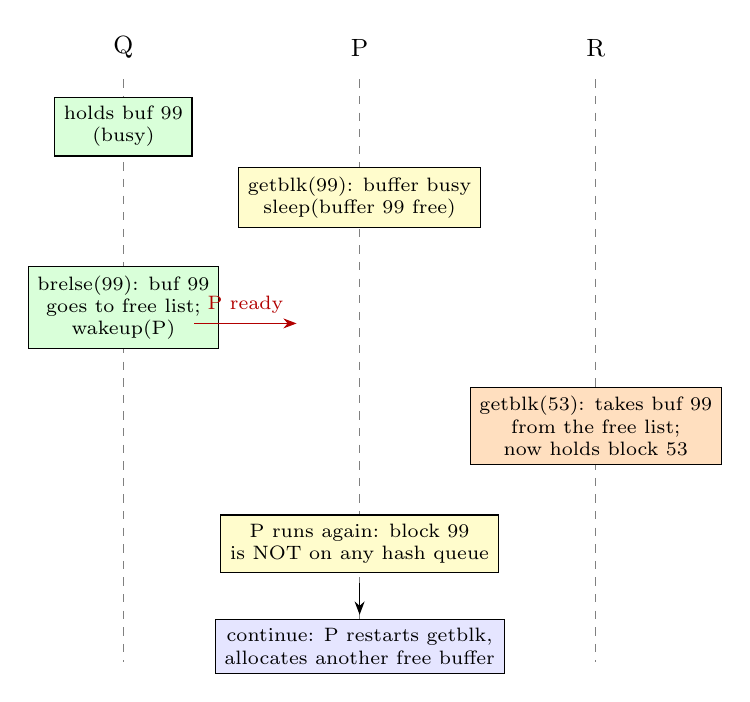
\begin{tikzpicture}[>=Stealth,font=\small]
\foreach \x/\n in {0/Q,3/P,6/R} { \node at (\x,0.4) {\n}; \draw[dashed,gray] (\x,0) -- (\x,-7.4); }
\node[draw,fill=green!15,font=\scriptsize,align=center] at (0,-0.6) {holds buf 99\\ (busy)};
\node[draw,fill=yellow!20,font=\scriptsize,align=center] at (3,-1.5) {getblk(99): buffer busy\\ sleep(buffer 99 free)};
\node[draw,fill=green!15,font=\scriptsize,align=center] at (0,-2.9) {brelse(99): buf 99\\ goes to free list;\\ wakeup(P)};
\draw[->,red!70!black] (0.9,-3.1) -- (2.2,-3.1) node[midway,above,font=\scriptsize,red!70!black]{P ready};
\node[draw,fill=orange!25,font=\scriptsize,align=center] at (6,-4.4) {getblk(53): takes buf 99\\ from the free list;\\ now holds block 53};
\node[draw,fill=yellow!20,font=\scriptsize,align=center] at (3,-5.9) {P runs again: block 99\\ is NOT on any hash queue};
\node[draw,fill=blue!10,font=\scriptsize,align=center] at (3,-7.2) {continue: P restarts getblk,\\ allocates another free buffer};
\draw[->] (3,-6.4) -- (3,-6.8);
\end{tikzpicture}
\end{document}
